% Ergebnisse und Analyse Diagramme.tex

\newcommand{\MergesortMaxArrayVerdoppelnMesswerte}{%
    \addplot[blue, mark=*] coordinates {
            (25000000,3017372600)
            (50000000,6315632400)
            (100000000,12777405700)
            (200000000,27203738300)
            (400000000,56441153000)
        };
    \addlegendentry{Mergesort Zufall}
}

\newcommand{\QuicksortMaxArrayVerdoppelnMesswerte}{%
    \addplot[green, mark=*] coordinates {
            (25000000,1528071600)
            (50000000,3248990900)
            (100000000,6653966800)
            (200000000,13778762100)
            (400000000,29074726600)
        };
    \addlegendentry{Quicksort Zufall}
}

\newcommand{\MergesortArrayVerdoppeln}{%
    \addplot[blue, mark=*] coordinates {
            (1,1000)
            (2,1300)
            (4,3100)
            (8,3200)
            (16,3500)
            (100,8700)
            (1000,97700)
            (2000,191700)
            (4000,354400)
            (8000,898800)
            (20000,1836000)
            (40000,3717200)
            (80000,7655300)
            (200000,19867700)
            (400000,40483400)
            (800000,83914700)
        };
    \addlegendentry{Mergesort}
}

\newcommand{\QuicksortArrayVerdoppeln}{%
    \addplot[green, mark=*] coordinates {
            (1,2700)
            (2,2800)
            (4,3100)
            (8,3800)
            (16,3300)
            (100,3000)
            (1000,34900)
            (2000,73100)
            (4000,148500)
            (8000,323600)
            (20000,826000)
            (40000,1777200)
            (80000,3888100)
            (200000,9835400)
            (400000,20598200)
            (800000,41432600)
        };
    \addlegendentry{Quicksort}
}

\newcommand{\QuicksortMaxArrayVerdoppelnMesswerteSortiert}{%
    \addplot[green!60!black, mark=*] coordinates {
            (25000000,165043900)
            (50000000,340924200)
            (100000000,726211400)
            (200000000,1550396900)
            (400000000,3130893200)
        };
    \addlegendentry{Quicksort Sortiert}
}

\newcommand{\MergesortgZufallG}{%
    \addplot[blue!, mark=*] coordinates {
            (1,1000)
            (2,1300)
            (4,3100)
            (8,3200)
            (10,4800)
            (16,3500)
            (100,8700)
            (1000,97700)
            (1200,115900)
            (2000,191700)
            (4000,354400)
            (8000,898800)
            (20000,1836000)
            (40000,3717200)
            (80000,7655300)
            (200000,19867700)
            (400000,40483400)
            (800000,83914700)
            (2000000,214959100)
            (4000000,441562800)
            (8000000,927314800)
            (25000000,3017372600)
            (40000000,5011540100)
            (50000000,6315632400)
            (100000000,12777405700)
            (200000000,27203738300)
            (400000000,56441153000)
        };
    \addlegendentry{Mergesort Zufall}
}

\newcommand{\QuicksortZufallG}{%
    \addplot[green, mark=*] coordinates {
            (1,2700)
            (2,2800)
            (4,3100)
            (8,3800)
            (10,400)
            (16,3300)
            (100,3000)
            (1000,34900)
            (1200,42900)
            (2000,73100)
            (4000,148500)
            (8000,323600)
            (20000,826000)
            (40000,1777200)
            (80000,3888100)
            (200000,9835400)
            (400000,20598200)
            (800000,41432600)
            (2000000,108526800)
            (4000000,218531900)
            (8000000,466862300)
            (25000000,1528071600)
            (40000000,2510531800)
            (50000000,3248990900)
            (100000000,6653966800)
            (200000000,13778762100)
            (400000000,29074726600)
        };
    \addlegendentry{Quicksort Zufall}
}

\newcommand{\MergesortgSortiertG}{%
    \addplot[blue!60!black, mark=*] coordinates {
            (1,200)
            (2,500)
            (4,1100)
            (8,1100)
            (10,900)
            (16,1600)
            (100,9100)
            (1000,63700)
            (1200,61900)
            (2000,109900)
            (4000,246500)
            (8000,502400)
            (20000,1676800)
            (40000,2321100)
            (80000,4356400)
            (200000,11443400)
            (400000,27704700)
            (800000,44349600)
            (2000000,119394700)
            (4000000,242919700)
            (8000000,504358000)
            (25000000,1609541400)
            (40000000,2733965500)
            (50000000,3314592200)
            (100000000,6854920900)
            (200000000,14495472700)
            (400000000,28117911500)
        };
    \addlegendentry{Mergesort Sortiert}
}

\newcommand{\QuicksortSortiertG}{%
    \addplot[green!70!black, mark=*] coordinates {
            (1,200)
            (2,300)
            (4,200)
            (8,200)
            (10,200)
            (16,300)
            (100,1000)
            (1000,4100)
            (1200,4800)
            (2000,8300)
            (4000,14800)
            (8000,34200)
            (20000,85300)
            (40000,179000)
            (80000,384300)
            (200000,1010200)
            (400000,2636000)
            (800000,4505800)
            (2000000,10849000)
            (4000000,22915200)
            (8000000,46914400)
            (25000000,165043900)
            (40000000,263361000)
            (50000000,340924200)
            (100000000,726211400)
            (200000000,1550396900)
            (400000000,3130893200)
        };
    \addlegendentry{Quicksort Sortiert}
}

\newcommand{\MergesortDupliziertG}{%
    \addplot[orange, mark=*] coordinates {
            (1,200)
            (2,500)
            (4,700)
            (8,1100)
            (10,1000)
            (16,1700)
            (100,8700)
            (1000,73500)
            (1200,90500)
            (2000,146000)
            (4000,298200)
            (8000,593500)
            (20000,1587000)
            (40000,3118300)
            (80000,6606800)
            (200000,15498400)
            (400000,31319100)
            (800000,64131400)
            (2000000,162417700)
            (4000000,328665200)
            (8000000,679938900)
            (25000000,2168311400)
            (40000000,3562459400)
            (50000000,4409952700)
            (100000000,8964155800)
            (200000000,18360003700)
            (400000000,38385447200)
        };
    \addlegendentry{Mergesort Dupliziert}
}

\newcommand{\QuicksortDupliziertG}{%
    \addplot[yellow, mark=*] coordinates {
            (1,100)
            (2,100)
            (4,200)
            (8,300)
            (10,300)
            (16,600)
            (100,3600)
            (1000,33300)
            (1200,31900)
            (2000,50000)
            (4000,98800)
            (8000,185300)
            (20000,599400)
            (40000,972900)
            (80000,1843800)
            (200000,5041800)
            (400000,9841900)
            (800000,19230300)
            (2000000,49799200)
            (4000000,102304100)
            (8000000,211552100)
            (25000000,666682700)
            (40000000,1061258600)
            (50000000,1314474600)
            (100000000,2723588000)
            (200000000,5627916700)
            (400000000,11116214800)
        };
    \addlegendentry{Quicksort Dupliziert}
}

\newcommand{\MergesortZufallSechzehnThreads}{%
    \addplot[orange, mark=*] coordinates {
            (10,354000)
            (16,622300)
            (100,545800)
            (1000,609200)
            (1200,713800)
            (2000,593500)
            (4000,594000)
            (8000,662300)
            (20000,870800)
            (40000,1087600)
            (80000,2306500)
            (200000,4510500)
            (400000,8740600)
            (4000000,73832700)
            (8000000,152378400)
            (25000000,501599400)
            (40000000,810861600)
            (50000000,1037010900)
            (100000000,2211188000)
            (200000000,4209308100)
            (400000000,8799988500)
        };
    \addlegendentry{Mergesort T16 Zufall}
}

\newcommand{\QuicksortZufallSechzehnThreads}{%
    \addplot[yellow, mark=*] coordinates {
            (10,377900)
            (16,313700)
            (100,524900)
            (1000,524500)
            (1200,578900)
            (2000,583600)
            (4000,574200)
            (8000,686200)
            (20000,758700)
            (40000,1247000)
            (80000,1893500)
            (200000,4607900)
            (400000,5819600)
            (800000,18598000)
            (2000000,32284600)
            (4000000,96927600)
            (8000000,122547100)
            (25000000,821245500)
            (40000000,848245300)
            (50000000,1514323900)
            (100000000,3122963800)
            (200000000,5156190000)
            (400000000,7499160500)
        };
    \addlegendentry{Quicksort T16 Zufall}
}

\newcommand{\MergesortSortiertSechzehnThreads}{%
    \addplot[blue!60!black, mark=*] coordinates {
            (10,403500)
            (16,593900)
            (100,572900)
            (1000,662300)
            (1200,564700)
            (2000,633600)
            (4000,580400)
            (8000,604700)
            (20000,626600)
            (40000,864100)
            (80000,1268400)
            (200000,3374300)
            (400000,8244500)
            (800000,10872700)
            (2000000,25563700)
            (4000000,47747700)
            (8000000,99499600)
            (25000000,328780100)
            (40000000,555196700)
            (50000000,694473100)
            (100000000,1430268000)
            (200000000,2881545300)
            (400000000,6027445700)
        };
    \addlegendentry{Mergesort T16 Sortiert}
}

\newcommand{\QuicksortSortiertSechzehnThreads}{%
    \addplot[green!70!black, mark=*] coordinates {
            (10,246500)
            (16,314600)
            (100,550300)
            (1000,548800)
            (1200,587200)
            (2000,580600)
            (4000,560700)
            (8000,606200)
            (20000,561800)
            (40000,614100)
            (80000,579200)
            (200000,768900)
            (400000,834600)
            (800000,1341300)
            (2000000,3583900)
            (4000000,6791500)
            (8000000,10824700)
            (25000000,36695400)
            (40000000,78544900)
            (50000000,72528700)
            (100000000,159059100)
            (200000000,352729600)
            (400000000,689215100)
        };
    \addlegendentry{Quicksort T16 Sortiert}
}

\newcommand{\MergesortFastSortiertSechzehnThreads}{%
    \addplot[orange, dashed, mark=*] coordinates {
            (10,365400)
            (16,606000)
            (100,583700)
            (1000,599500)
            (1200,555200)
            (2000,598800)
            (4000,583000)
            (8000,594000)
            (20000,667800)
            (40000,878700)
            (80000,1324500)
            (200000,2638400)
            (400000,5884600)
            (800000,11399600)
            (2000000,24971500)
            (4000000,48312400)
            (8000000,103352500)
            (25000000,331426900)
            (40000000,551960100)
            (50000000,674324000)
            (100000000,1425747800)
            (200000000,2786237400)
            (400000000,5812322100)
        };
    \addlegendentry{Mergesort T16 FastSortiert}
}

\newcommand{\QuicksortFastSortiertSechzehnThreads}{%
    \addplot[yellow, dashed, mark=*] coordinates {
            (10,315000)
            (16,322200)
            (100,578700)
            (1000,526100)
            (1200,535400)
            (2000,558500)
            (4000,565700)
            (8000,587100)
            (20000,635800)
            (40000,624200)
            (80000,598200)
            (200000,705000)
            (400000,821100)
            (800000,1503500)
            (2000000,3730500)
            (4000000,6941600)
            (8000000,12923300)
            (25000000,34955000)
            (40000000,60236700)
            (50000000,81307600)
            (100000000,161113800)
            (200000000,341155900)
            (400000000,665058900)
        };
    \addlegendentry{Quicksort T16 FastSortiert}
}


\newcommand{\MergesortZufallSechzehnWorkerThreads}{%
    \addplot[orange, mark=*] coordinates {
            (1,559900)
            (2,545700)
            (4,1187400)
            (8,599100)
            (10,582400)
            (16,711700)
            (100,648900)
            (1000,657900)
            (1200,646400)
            (2000,693400)
            (4000,720800)
            (8000,751700)
            (20000,1118300)
            (40000,1491500)
            (80000,2242200)
            (200000,4781300)
            (400000,8867800)
            (800000,17266800)
            (2000000,44136100)
            (4000000,97449500)
            (8000000,203663400)
            (25000000,547983700)
            (40000000,980483500)
            (50000000,1164662400)
            (100000000,2629364700)
            (200000000,5479476700)
            (400000000,10859430800)
        };
    \addlegendentry{Mergesort WT16 Zufall}
}

\newcommand{\QuicksortZufallSechzehnWorkerThreads}{%
    \addplot[yellow, mark=*] coordinates {
            (1,575600)
            (2,657500)
            (4,648600)
            (8,640600)
            (10,532200)
            (16,822100)
            (100,657600)
            (128,645200)
            (256,538100)
            (400,678900)
            (1000,647600)
            (1024,659300)
            (1200,637400)
            (2000,630100)
            (4000,618400)
            (4096,779800)
            (8000,792800)
            (20000,732100)
            (40000,923300)
            (80000,1325900)
            (200000,2461700)
            (400000,3817200)
            (800000,7220000)
            (2000000,17698800)
            (4000000,32127800)
            (8000000,64708400)
            (25000000,198604300)
            (40000000,327429200)
            (50000000,437240700)
            (100000000,866735700)
            (200000000,1790304900)
            (400000000,3836458700)
        };
    \addlegendentry{Quicksort WT16 Zufall}
}

\newcommand{\MergesortSortiertSechzehnWorkerThreads}{%
    \addplot[blue!60!black, mark=*] coordinates {
            (1,599500)
            (2,650500)
            (4,529400)
            (8,606000)
            (10,573100)
            (16,652400)
            (100,636400)
            (1000,721400)
            (1200,755300)
            (2000,671500)
            (4000,572300)
            (8000,612900)
            (20000,761600)
            (40000,1002800)
            (80000,1667700)
            (200000,2967900)
            (400000,5937500)
            (800000,10890500)
            (2000000,27398900)
            (4000000,57325000)
            (8000000,109365800)
            (25000000,353182000)
            (40000000,654028700)
            (50000000,693445000)
            (100000000,1578904700)
            (200000000,3169421700)
            (400000000,6304755900)
        };
    \addlegendentry{Mergesort WT16 Sortiert}
}

\newcommand{\QuicksortSortiertSechzehnWorkerThreads}{%
    \addplot[green!70!black, mark=*] coordinates {
            (1,604400)
            (2,590100)
            (4,658600)
            (8,654200)
            (10,736600)
            (16,524700)
            (100,640700)
            (128,739400)
            (256,618400)
            (400,625500)
            (1000,594500)
            (1024,619900)
            (1200,822800)
            (2000,671400)
            (4000,659000)
            (4096,664400)
            (8000,626200)
            (20000,628500)
            (40000,771700)
            (80000,718900)
            (200000,947300)
            (400000,1188400)
            (800000,1371400)
            (2000000,2813200)
            (4000000,5369900)
            (8000000,9791600)
            (25000000,36718200)
            (40000000,61933000)
            (50000000,80577100)
            (100000000,176064800)
            (200000000,375860500)
            (400000000,766518900)
        };
    \addlegendentry{Quicksort WT16 Sortiert}
}

\newcommand{\MergesortStringZufallG}{%
    \addplot[blue!, mark=*] coordinates {
            (1,2200)
            (2,500)
            (4,900)
            (8,2600)
            (10,3300)
            (16,7700)
            (100,37000)
            (1000,388800)
            (1200,424700)
            (2000,890100)
            (4000,1475200)
            (8000,4087500)
            (20000,9995800)
            (40000,17852300)
            (80000,37861200)
            (200000,101671300)
            (400000,213857100)
            (800000,452853700)
            (2000000,1204999800)
            (2500000,1507792900)
            (4000000,2486550700)
            (5000000,3184070600)
            (8000000,5233667300)
            (10000000,6707397200)
            (20000000,13948479700)
            (40000000,28775560100)
            (80000000,60049783100)
        };
    \addlegendentry{Mergesort Zufall}
}

\newcommand{\QuicksortStringZufallG}{%
    \addplot[green, mark=*] coordinates {
            (1,100)
            (2,300)
            (4,400)
            (8,900)
            (10,1200)
            (16,1600)
            (100,12500)
            (1000,154000)
            (1200,187200)
            (2000,342700)
            (4000,721000)
            (8000,1536600)
            (20000,4365600)
            (40000,9131800)
            (80000,18232700)
            (200000,49089400)
            (400000,103713700)
            (800000,213115000)
            (2000000,572717300)
            (2500000,733376100)
            (4000000,1197172500)
            (5000000,1514452900)
            (8000000,2500057800)
            (10000000,3132198100)
            (20000000,6566592900)
            (40000000,13756918200)
            (80000000,28743478100)
        };
    \addlegendentry{Quicksort Zufall}
}

\newcommand{\MergesortStringZufallSechzehnThreads}{%
    \addplot[orange, mark=*] coordinates {
            (10,411100)
            (16,549000)
            (100,624300)
            (1000,646800)
            (1200,657800)
            (2000,724700)
            (4000,935800)
            (8000,1263900)
            (20000,2344300)
            (40000,4762100)
            (80000,7690800)
            (200000,20141900)
            (800000,86828400)
            (2000000,248630500)
            (2500000,329765800)
            (4000000,515049900)
            (5000000,666755800)
            (8000000,1086652400)
            (10000000,1395927400)
            (20000000,2900787400)
            (40000000,6080535900)
            (80000000,12570922600)
        };
    \addlegendentry{Mergesort T16 Zufall}
}

\newcommand{\QuicksortStringZufallSechzehnWorkerThreads}{%
    \addplot[yellow, mark=*] coordinates {
            (1,724900)
            (2,753600)
            (4,648600)
            (8,676200)
            (10,776500)
            (16,607900)
            (100,650700)
            (1000,1252600)
            (1200,763800)
            (2000,887000)
            (4000,1288700)
            (8000,1103000)
            (20000,2193300)
            (40000,2991400)
            (80000,4466500)
            (200000,9812000)
            (400000,22211500)
            (800000,38384700)
            (2000000,82175500)
            (2500000,128736600)
            (4000000,171978300)
            (5000000,227100100)
            (8000000,397251200)
            (10000000,459421100)
            (20000000,908786000)
            (40000000,1945039800)
            (80000000,4226169900)
        };
    \addlegendentry{Quicksort WT16 Zufall}
}

\newcommand{\MergesortStringSortiertSechzehnThreads}{%
    \addplot[blue!60!black, mark=*] coordinates {
            (10,397100)
            (16,591000)
            (100,1171700)
            (1000,603100)
            (1200,605100)
            (2000,687000)
            (4000,859200)
            (8000,1001400)
            (20000,1618900)
            (40000,3287600)
            (80000,6216100)
            (200000,15462400)
            (400000,32776600)
            (800000,62271800)
            (2000000,186974300)
            (2500000,238313300)
            (4000000,410541100)
            (5000000,528350300)
            (8000000,855291600)
            (10000000,1116975800)
            (20000000,2325526600)
            (40000000,4935200900)
            (80000000,10465589300)
        };
    \addlegendentry{Mergesort T16 Sortiert}
}

\newcommand{\QuicksortStringSortiertSechzehnWorkerThreads}{%
    \addplot[green!70!black, mark=*] coordinates {
            (1,630800)
            (2,583600)
            (4,644200)
            (8,631500)
            (10,566100)
            (16,637800)
            (100,547200)
            (1000,696200)
            (1200,679800)
            (2000,895800)
            (4000,971100)
            (8000,1016100)
            (20000,1646700)
            (40000,2968900)
            (80000,3243600)
            (200000,7051000)
            (400000,22824200)
            (800000,28260800)
            (2000000,69035900)
            (2500000,204315100)
            (4000000,238897600)
            (5000000,238713100)
            (8000000,345098500)
            (10000000,345748500)
            (20000000,796731800)
            (40000000,2713229900)
            (80000000,3923277000)
        };
    \addlegendentry{Quicksort WT16 Sortiert}
}

\newcommand{\MergesortWZufallStrongScaling}{%
    % 400M
    \addplot[blue, mark=*] coordinates {
            (1,54890541400)
            (2,28593265600)
            (4,19979246500)
            (8,13853421700)
            % (15,10312207800)
            (16,10859430800)
            % (17,10948184100)
            % (18,10749886000)
            (32,9307306300)
            (64,9071268100)
            (128,9230853500)
            (256,9256567600)
            (1024,9894312600)
            (4096,13091277800)
            (8192,21360609200)
            (16384,22809325900)
        };
    \addlegendentry{Mergesort Zufall}
}

\newcommand{\QuicksortWZufallStrongScaling}{%
    % 400M
    \addplot[green, mark=*] coordinates {
            (1,28735107800)
            (2,15226912200)
            (4,8622861300)
            (8,5325432800)
            % (15,3934768300)
            (16,3836458700)
            % (17,3788112100)
            % (18,3806813500)
            (32,3891350600)
            (64,4281481700)
            (128,4303495100)
            (256,4368919100)
            (1024,4551948300)
            (4096,6646592400)
            (8192,11730603100)
            (16384,12841474600)
        };
    \addlegendentry{Quicksort Zufall}
}

\newcommand{\MergesortWZufallWeakScaling}{%
    % Threads und Länge verdoppeln
    \addplot[blue, mark=*] coordinates {
            (1,3053568900)
            (2,3599563800)
            (4,4548506700)
            (8,6766294600)
            (16,10859430800)
        };
    \addlegendentry{Mergesort Zufall}
}

\newcommand{\QuicksortWZufallWeakScaling}{%
    % Threads und Länge verdoppeln
    \addplot[green, mark=*] coordinates {
            (1,1558438200)
            (2,1700040600)
            (4,1972159600)
            (8,2201854900)
            (16,3836458700)
        };
    \addlegendentry{Quicksort Zufall}
}

\newcommand{\MergesortZufallWeakScaling}{%
    % Threads und Länge verdoppeln
    \addplot[blue, mark=*] coordinates {
            (1,3015068500)
            (2,3420072500)
            (4,3881172000)
            (8,5347002100)
            (16,8799988500)
        };
    \addlegendentry{Mergesort Zufall}
}

\newcommand{\QuicksortZufallWeakScaling}{%
    % Threads und Länge verdoppeln
    \addplot[green, mark=*] coordinates {
            (1,1541334700)
            (2,2792193000)
            (4,3627494500)
            (8,9023601000)
            (16,7499160500)
        };
    \addlegendentry{Quicksort Zufall}
}

\newcommand{\MergesortZufallStrongScaling}{%
    % 400M
    \addplot[blue, mark=*] coordinates {
            (1,56291760800)
            (2,29452091000)
            (4,16471478900)
            (8,10978147600)
            (16,8799988500)
            (2^5,9135850400)
            (2^6,9686368700)
            (2^7,9288907600)
            (2^8,9163394200)
            (2^9,9243936800)
            (2^10,9234824900)
            (2^11,9214304700)
            (2^12,9410109100)
            (2^13,9530975800)
            (2^14,9652868400)
        };
    \addlegendentry{Mergesort Zufall}
}

\newcommand{\QuicksortZufallStrongScaling}{%
    % 400M
    \addplot[green, mark=*] coordinates {
            (1,29150929400)
            (2,16718432700)
            (4,11842161000)
            (8,11334038600)
            (16,7499160500)
            (2^5,5546354600)
            (2^6,4761041600)
            (2^7,4713548700)
            (2^8,4234104700)
            (2^9,4256117200)
            (2^10,4022481400)
            (2^11,4233575500)
            (2^12,3948265600)
            (2^13,3924137200)
            (2^14,4034757100)
        };
    \addlegendentry{Quicksort Zufall}
}

\newcommand{\MergesortStringZufallStrongScaling}{%
    % 40M
    \addplot[blue, mark=*] coordinates {
            (1,28745673200)
            (2,15141553600)
            (4,9275936100)
            (8,6504576100)
            (16,6080535900)
            (2^5,5727016500)
            (2^6,5895803400)
            (2^7,5898748700)
            (2^8,5981683100)
            (2^9,6050864000)
            (2^10,6184462200)
            (2^11,6332948900)
            (2^12,6490905200)
            (2^13,6578309000)
            (2^14,6783299000)
        };
    \addlegendentry{Mergesort T Zufall String}
}

\newcommand{\QuicksortWStringZufallStrongScaling}{%
    % 40M
    \addplot[green, mark=*] coordinates {
            (1,13932820500)
            (2,7266935300)
            (4,4008472800)
            (8,2603287000)
            (16,1945039800)
            (32,2083285400)
            (64,2142911600)
            (128,2212413900)
            (256,2268350200)
            (1024,2582845900)
            (4096,3933490900)
            (8192,9109748600)
            (16384,11769250700)
        };
    \addlegendentry{Quicksort WT Zufall String}
}

\newcommand{\MergesortStringZufallWeakScaling}{%
    % Threads und Länge verdoppeln
    % 2.5M
    \addplot[blue, mark=*] coordinates {
            (1,1496391700)
            (2,1675389600)
            (4,2137721000)
            (8,3222821900)
            (16,6080535900)
        };
    \addlegendentry{Mergesort T Zufall String}
}

\newcommand{\QuicksortStringWZufallWeakScaling}{%
    % Threads und Länge verdoppeln
    % 2.5M
    \addplot[green, mark=*] coordinates {
            (1,730048100)
            (2,798399500)
            (4,934075300)
            (8,1200469500)
            (16,1945039800)
        };
    \addlegendentry{Quicksort WT Zufall String}
}

\newcommand{\MergesortTInitZeiten}{%
    % 16
    \addplot[blue, mark=*] coordinates {
            (1,2800)
            (2,811700)
            (4,209500)
            (8,326800)
            (16,622300)
        };
    \addlegendentry{Mergesort T Zufall}
}

\newcommand{\QuicksortTInitZeiten}{%
    % 16
    \addplot[green, mark=*] coordinates {
            (1,500)
            (2,91400)
            (4,171200)
            (8,306500)
            (16,314600)
        };
    \addlegendentry{Quicksort T Sortiert}
}

\newcommand{\MergesortWTInitZeiten}{%
    % 16
    \addplot[orange, mark=*] coordinates {
            (1,2500)
            (2,118800)
            (4,138600)
            (8,284500)
            % (15,459800)
            (16,711700)
            % (17,644600)
            % (18,623600s)
            (32,1198800)
            (64,2273300)
            (128,4874300)
            (256,8935300)
            (1024,41633200)
            (4096,171494600)
            (8192,326434900)
            (16384,662938200)
        };
    \addlegendentry{Mergesort WT Zufall}
}

\newcommand{\QuicksortWTInitZeiten}{%
    % 16
    \addplot[yellow, mark=*] coordinates {
            (1,133300)
            (2,149400)
            (4,258900)
            (8,509000)
            % (15,589600)
            (16,822100)
            % (17,904000)
            % (18,768500)
            (32,1458000)
            (64,2998300)
            (128,4966400)
            (256,11230100)
            (1024,43468700)
            (4096,212968900)
            (8192,361395500)
            (16384,678190600)
        };
    \addlegendentry{Quicksort WT Zufall}
}

\newcommand{\TheorieStrongScaling}[2]{%
    \pgfmathsetmacro{\n}{#1} % 400000000
    \pgfmathsetmacro{\faktor}{#2} % 2.5
    \addplot[
        black,
        dashed,
        % domain=1:2^14,
        % samples=100
    ]
    % T(n,e) = n * 2 ( 1 - 1 / ( 2 ^ e ) ) + (n/2^e)*log2( (n/2^e)) + (n/2^e)
    coordinates {
            (1, { (2*\n*(1-1/(2^0)) + (\n/(2^0))*ln(\n/(2^0))/ln(2) + (\n/(2^0)))*\faktor })
            (2, { (2*\n*(1-1/(2^1)) + (\n/(2^1))*ln(\n/(2^1))/ln(2) + (\n/(2^1)))*\faktor })
            (4, { (2*\n*(1-1/(2^2)) + (\n/(2^2))*ln(\n/(2^2))/ln(2) + (\n/(2^2)))*\faktor })
            (8, { (2*\n*(1-1/(2^3)) + (\n/(2^3))*ln(\n/(2^3))/ln(2) + (\n/(2^3)))*\faktor })
            (16, { (2*\n*(1-1/(2^4)) + (\n/(2^4))*ln(\n/(2^4))/ln(2) + (\n/(2^4)))*\faktor })
            (32, { (2*\n*(1-1/(2^5)) + (\n/(2^5))*ln(\n/(2^5))/ln(2) + (\n/(2^5)))*\faktor })
            (64, { (2*\n*(1-1/(2^6)) + (\n/(2^6))*ln(\n/(2^6))/ln(2) + (\n/(2^6)))*\faktor })
            (128, { (2*\n*(1-1/(2^7)) + (\n/(2^7))*ln(\n/(2^7))/ln(2) + (\n/(2^7)))*\faktor })
            (256, { (2*\n*(1-1/(2^8)) + (\n/(2^8))*ln(\n/(2^8))/ln(2) + (\n/(2^8)))*\faktor })
            (512, { (2*\n*(1-1/(2^9)) + (\n/(2^9))*ln(\n/(2^9))/ln(2) + (\n/(2^9)))*\faktor })
            (1024, { (2*\n*(1-1/(2^10)) + (\n/(2^10))*ln(\n/(2^10))/ln(2) + (\n/(2^10)))*\faktor })
            (2048, { (2*\n*(1-1/(2^11)) + (\n/(2^11))*ln(\n/(2^11))/ln(2) + (\n/(2^11)))*\faktor })
            (4096, { (2*\n*(1-1/(2^12)) + (\n/(2^12))*ln(\n/(2^12))/ln(2) + (\n/(2^12)))*\faktor })
            (8192, { (2*\n*(1-1/(2^13)) + (\n/(2^13))*ln(\n/(2^13))/ln(2) + (\n/(2^13)))*\faktor })
            (16384, { (2*\n*(1-1/(2^14)) + (\n/(2^14))*ln(\n/(2^14))/ln(2) + (\n/(2^14)))*\faktor })
        };
    % \addlegendentry{Theoretische Laufzeit ($\times \text{\faktor}$)}
}

\newcommand{\TheorieWeakScaling}[1]{%
    % \pgfmathsetmacro{\nzero}{25000000}
    \pgfmathsetmacro{\faktor}{#1} % 2.5
    \addplot[
        black,
        dashed,
        % domain=1:16,
        % samples=100
    ]
    % T(n,e) = n * 2 ( 1 - 1 / ( 2 ^ e ) ) + (n/2^e)*log2( (n/2^e)) + (n/2^e)
    coordinates {
            (1, 639385619 * \faktor)
            (2, 689385619 * \faktor)
            (4, 789385619 * \faktor)
            (8, 989385619 * \faktor)
            (16, 1389385619 * \faktor)
        };
    % \addlegendentry{Theoretische Laufzeit ($\times \text{\faktor}$)}
}

\newcommand{\TheorieWeakScalingB}[1]{%
    % \pgfmathsetmacro{\nzero}{2500000}
    \pgfmathsetmacro{\faktor}{#1} % 2.5
    \addplot[
        black,
        dashed,
        % domain=1:16,
        % samples=100
    ]
    % T(n,e) = n * 2 ( 1 - 1 / ( 2 ^ e ) ) + (n/2^e)*log2( (n/2^e)) + (n/2^e)
    coordinates {
            (1, 55719250 * \faktor)
            (2, 60719250 * \faktor)
            (4, 70719250 * \faktor)
            (8, 90719250 * \faktor)
            (16, 130719250 * \faktor)
        };
    % \addlegendentry{Theoretische Laufzeit ($\times \text{\faktor}$)}
}

\newcommand{\GrundlegendeLaufzeitenAbhaengigVonDerArraygroesseDiagrammA}{%
    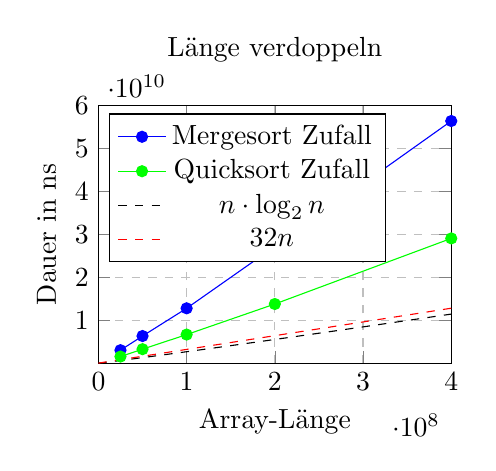
\begin{tikzpicture}
        \begin{axis}[
                title style={yshift=1.5ex},
                width=0.5\textwidth,
                height=0.4\textwidth,
                xlabel={Array-Länge},
                ylabel={Dauer in ns},
                title={Länge verdoppeln},
                xmin=0, xmax=4 * 10^8,
                ymin=0, ymax=6*10^10,
                grid=both,
                grid style=dashed,
                legend pos=north west,
                ytick={1*10^10,2*10^10,3*10^10,4*10^10,5*10^10,6*10^10},
                % xtick={2^21,2^23,2^24,2^25},
                % xticklabels={$2^{21}$, $2^{23}$, $2^{24}$, $2^{25}$},
                % scaled x ticks=false,
                % scaled y ticks=false,
            ]
            \MergesortMaxArrayVerdoppelnMesswerte
            \QuicksortMaxArrayVerdoppelnMesswerte
            % n*log2(n)
            \addplot[black, dashed,domain=1:4e8, samples=100] {x*log2(x)};
            \addlegendentry{$n \cdot \log_2 n$}
            % n
            \addplot[red, dashed,domain=1:4e8, samples=100] {32*x};
            \addlegendentry{$32n$}
            % % log2(n)
            % \addplot[green, domain=1e7:4e8, samples=100] {log2(x)};
            % \addlegendentry{$\log_2 n$}
        \end{axis}
    \end{tikzpicture}%
}

\newcommand{\GrundlegendeLaufzeitenAbhaengigVonDerArraygroesseDiagrammB}{%
    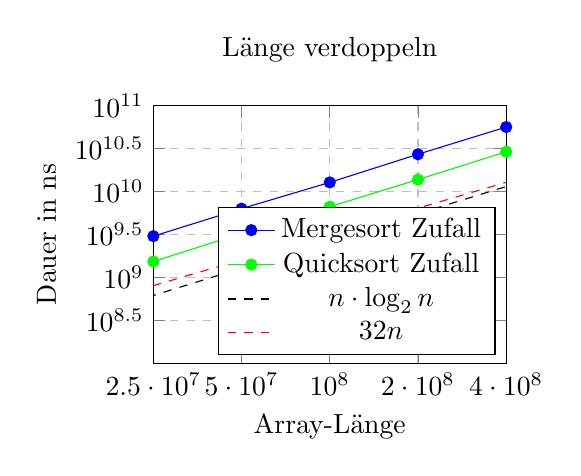
\begin{tikzpicture}
        \begin{axis}[
                title style={yshift=1.5ex},
                width=0.5\textwidth,
                height=0.4\textwidth,
                xlabel={Array-Länge},
                ylabel={Dauer in ns},
                title={Länge verdoppeln},
                xmin=2.5*10^7, xmax=4*10^8,
                ymin=10^8, ymax=1*10^11,
                grid=both,
                grid style=dashed,
                legend pos=south east,
                xmode=log,
                log basis x=10,
                xtick=data,
                xticklabels={$2.5\cdot10^7$, $5\cdot10^7$, $10^8$, $2\cdot10^8$, $4\cdot10^8$},
                ymode=log,
                log basis y=10,
                % ytick=data,
                ytick={10^8.5,10^9,1*10^9.5,1*10^10,1*10^10.5,1*10^11},
                minor y tick num=9,
                yminorgrids=true,
                % xtick={2^21,2^23,2^24,2^25},
                % xticklabels={$2^{21}$, $2^{23}$, $2^{24}$, $2^{25}$},
                % scaled x ticks=false,
                % scaled y ticks=false,
            ]
            \MergesortMaxArrayVerdoppelnMesswerte
            \QuicksortMaxArrayVerdoppelnMesswerte
            % n*log2(n)
            \addplot[black, dashed,domain=1e7:4e8, samples=100] {x*log2(x)};
            \addlegendentry{$n \cdot \log_2 n$}
            % n
            \addplot[red, dashed,domain=1:4e8, samples=100] {32*x};
            \addlegendentry{$32n$}
            % % 64*x - 1000000000
            % \addplot[gray, dashed,domain=2*10^7:4e8, samples=100] {64*x - 10^9};
            % \addlegendentry{$64 \cdot n - 10^9$}
        \end{axis}
    \end{tikzpicture}%
}

\newcommand{\GrundlegendeLaufzeitenAbhaengigVonDerArraygroesseDiagrammC}{%
    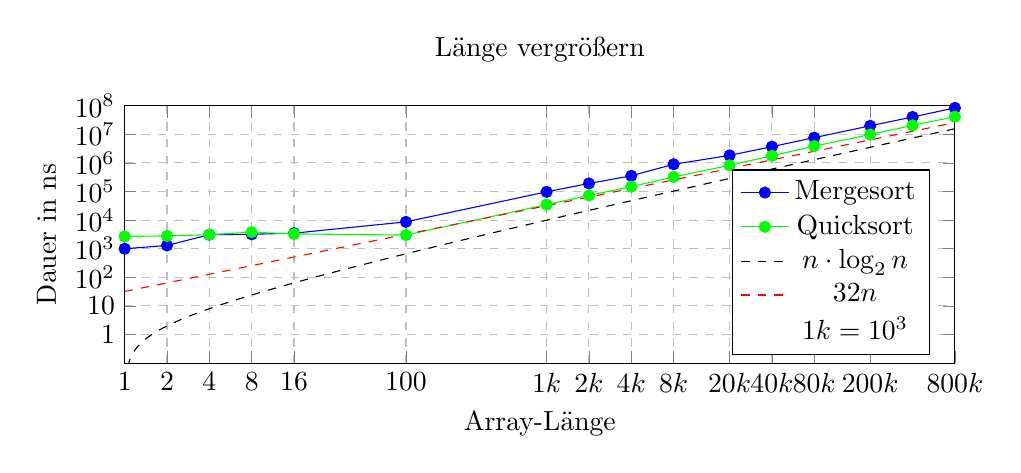
\begin{tikzpicture}
        \begin{axis}[
                title style={yshift=1.5ex},
                width=1\textwidth,
                height=0.4\textwidth,
                xlabel={Array-Länge},
                ylabel={Dauer in ns},
                title={Länge vergrößern},
                xmin=1, xmax=800000,
                ymin=0.1, ymax=1*10^8,
                grid=both,
                grid style=dashed,
                legend pos=south east,
                xmode=log,
                log basis x=10,
                %xtick=data,
                xtick={1,2,4,8,16,100,1000,2000,4000,8000,20000,40000,80000,200000,800000},
                xticklabels={
                        $1$,$2$,$4$,$8$,$16$,
                        $100$,$1k$,
                        $2k$,$4k$,$8k$,
                        $20k$,$40k$,$80k$,
                        $200k$,$800k$
                    },
                ymode=log,
                log basis y=10,
                ytick={1,10,10^2,10^3,10^4,10^5,10^6,10^7,10^8},
                yticklabels={$1$,$10$,$10^{2}$,$10^{3}$,$10^{4}$,$10^{5}$,$10^{6}$,$10^{7}$,$10^{8}$},
                % scaled x ticks=false,
                % scaled y ticks=false,
            ]
            \MergesortArrayVerdoppeln
            \QuicksortArrayVerdoppeln
            % n*log2(n)
            \addplot[black, dashed,domain=1:800000, samples=1000] {x*log2(x)};
            \addlegendentry{$n \cdot \log_2 n$}
            % n
            \addplot[red, dashed,domain=1:800000, samples=100] {32*x};
            \addlegendentry{$32n$}
            \addlegendimage{empty legend}
            \addlegendentry{$1k = 10^3$}
        \end{axis}
    \end{tikzpicture}%
}

\newcommand{\EinflussDesListentypsDiagrammA}{%
    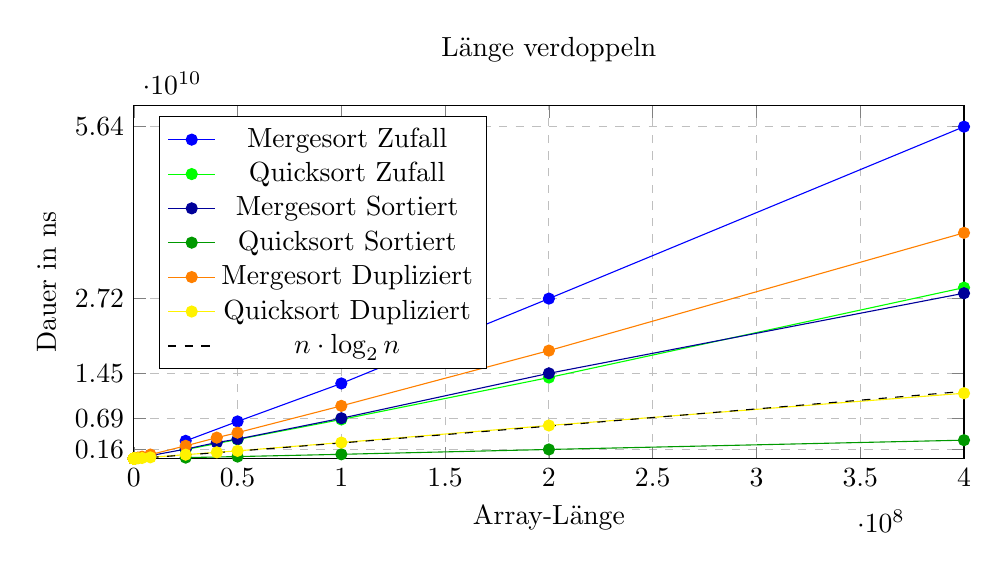
\begin{tikzpicture}
        \begin{axis}[
                title style={yshift=1.5ex},
                width=1\textwidth,
                height=0.5\textwidth,
                xlabel={Array-Länge},
                ylabel={Dauer in ns},
                title={Länge verdoppeln},
                xmin=0, xmax=4 * 10^8,
                ymin=0, ymax=6*10^10,
                grid=both,
                grid style=dashed,
                legend pos=north west,
                ytick={1609541400,6854920900,14495472700,27203738300,56441153000},
                % xtick={2^21,2^23,2^24,2^25},
                % xticklabels={$2^{21}$, $2^{23}$, $2^{24}$, $2^{25}$},
                % scaled x ticks=false,
                % scaled y ticks=false,
            ]
            \MergesortMaxArrayVerdoppelnMesswerte
            \QuicksortMaxArrayVerdoppelnMesswerte
            \MergesortgSortiertG
            \QuicksortMaxArrayVerdoppelnMesswerteSortiert
            \MergesortDupliziertG
            \QuicksortDupliziertG
            % n*log2(n)
            \addplot[black, dashed,domain=1:4e8, samples=100] {x*log2(x)};
            \addlegendentry{$n \cdot \log_2 n$}
        \end{axis}
    \end{tikzpicture}%
}

\newcommand{\EinflussDesListentypsDiagrammB}{%
    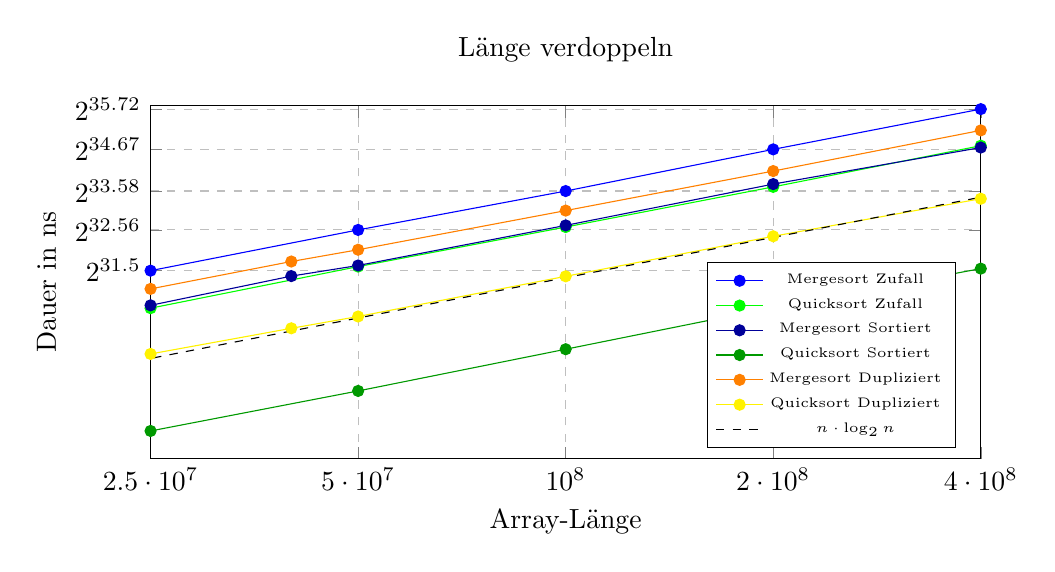
\begin{tikzpicture}
        \begin{axis}[
                title style={yshift=1.5ex},
                width=1\textwidth,
                height=0.5\textwidth,
                xlabel={Array-Länge},
                ylabel={Dauer in ns},
                title={Länge verdoppeln},
                xmin=2.5*10^7, xmax=4*10^8,
                ymin=10^8, ymax=6*10^10,
                grid=both,
                grid style=dashed,
                legend pos=south east,
                legend style={font=\tiny},
                xmode=log,
                log basis x=10,
                xtick=data,
                xticklabels={$2.5\cdot10^7$, $5\cdot10^7$, $10^8$, $2\cdot10^8$, $4\cdot10^8$},
                ymode=log,
                log basis y=2,
                ytick=data,
                % xtick={2^21,2^23,2^24,2^25},
                % xticklabels={$2^{21}$, $2^{23}$, $2^{24}$, $2^{25}$},
                % scaled x ticks=false,
                % scaled y ticks=false,
            ]
            \MergesortMaxArrayVerdoppelnMesswerte
            \QuicksortMaxArrayVerdoppelnMesswerte
            \MergesortgSortiertG
            \QuicksortMaxArrayVerdoppelnMesswerteSortiert
            \MergesortDupliziertG
            \QuicksortDupliziertG
            % n*log2(n)
            \addplot[black, dashed,domain=1e7:4e8, samples=100] {x*log2(x)};
            \addlegendentry{$n \cdot \log_2 n$}
        \end{axis}
    \end{tikzpicture}%
}

\newcommand{\EinflussDesListentypsDiagrammC}{%
    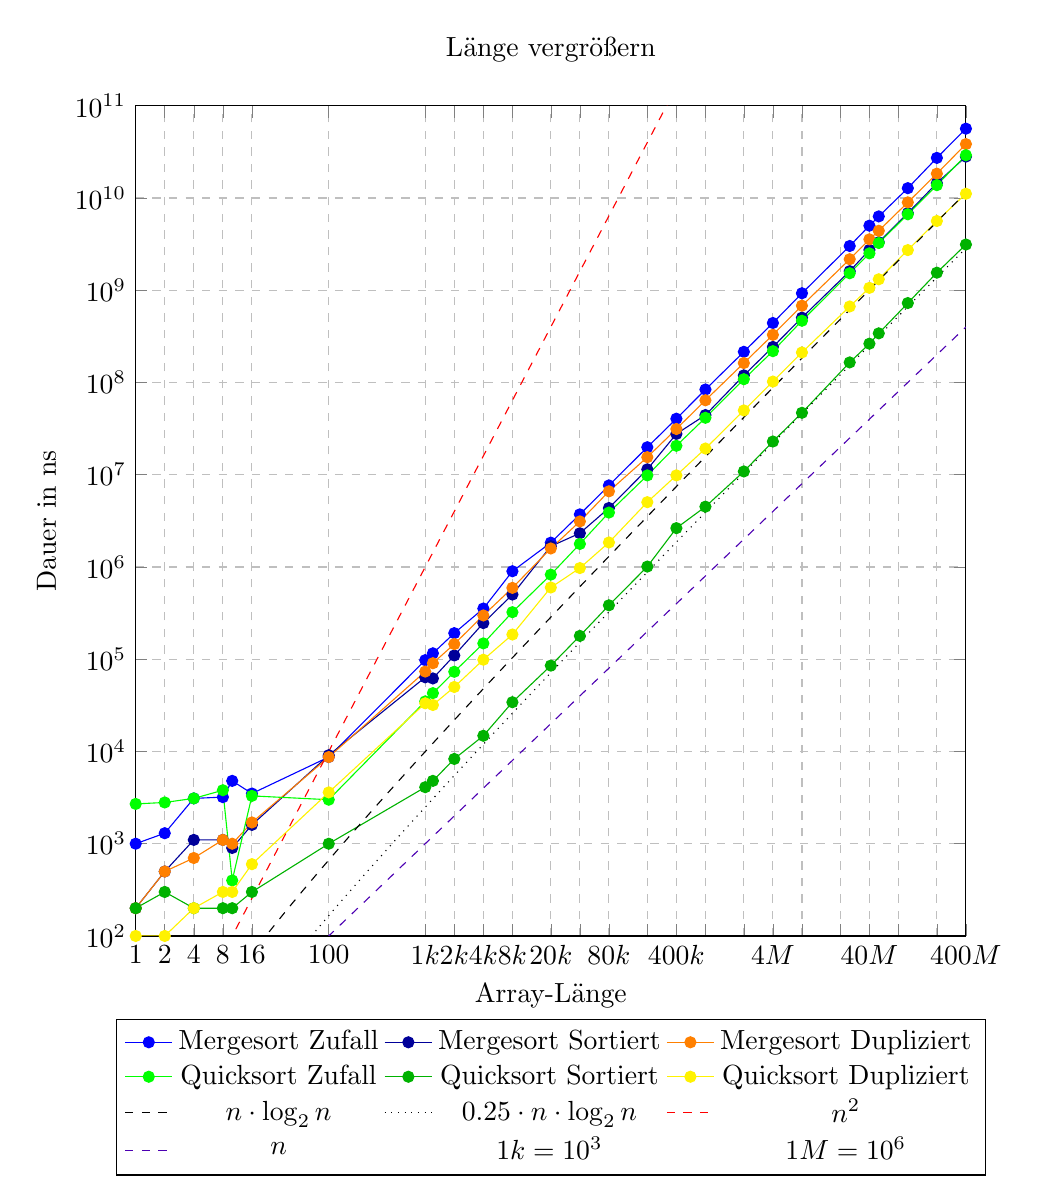
\begin{tikzpicture}
        \begin{axis}[
                title style={yshift=1.5ex},
                width=1\textwidth,
                height=1\textwidth,
                xlabel={Array-Länge},
                ylabel={Dauer in ns},
                title={Länge vergrößern},
                xmin=1, xmax=400000000,
                ymin=100, ymax=1*10^11,
                grid=both,
                grid style=dashed,
                % legend pos=south east,
                legend style={
                        at={(0.5,-0.1)},
                        anchor=north,
                        legend columns=3
                    },
                xmode=log,
                log basis x=10,
                %xtick=data,
                xtick={1,2,4,8,16,100,1000,2000,4000,8000,20000,40000,80000,200000,400000,800000,2000000,4000000,8000000,20000000,40000000,80000000,200000000,400000000},
                xticklabels={
                        $1$,$2$,$4$,$8$,$16$,
                        $100$,$1k$,
                        $2k$,$4k$,$8k$,
                        $20k$,$$,$80k$,
                            $ $,$400k$,$ $,
                            $ $,$4M$,$$,
                            $$,$40M$,$$,
                            $$,$400M$,$$
                    },
                ymode=log,
                log basis y=10,
                ytick={1,10,10^2,10^3,10^4,10^5,10^6,10^7,10^8,10^9,10^10,10^11},
                yticklabels={$1$,$10$,$10^{2}$,$10^{3}$,$10^{4}$,$10^{5}$,$10^{6}$,$10^{7}$,$10^{8}$,$10^{9}$,$10^{10}$,$10^{11}$}
                % scaled x ticks=false,
                % scaled y ticks=false,
            ]
            \MergesortgZufallG
            \MergesortgSortiertG
            \MergesortDupliziertG
            \QuicksortZufallG
            \QuicksortSortiertG
            \QuicksortDupliziertG
            % n*log2(n)
            \addplot[black, dashed,domain=1:400000000, samples=1000] {x*log2(x)};
            \addlegendentry{$n \cdot \log_2 n$}
            % 0.25*n*log2(n)
            \addplot[black, dotted,domain=1:400000000, samples=1000] {0.25*x*log2(x)};
            \addlegendentry{$0.25 \cdot n \cdot \log_2 n$}
            % n^2
            \addplot[red, dashed,domain=1:4e8, samples=100] {x*x};
            \addlegendentry{$n^2$}
            % n
            \addplot[blue!70!red, dashed,domain=1:4e8, samples=100] {x};
            \addlegendentry{$n$}
            \addlegendimage{empty legend}
            \addlegendentry{$1k = 10^3$}
            \addlegendimage{empty legend}
            \addlegendentry{$1M = 10^6$}
        \end{axis}
    \end{tikzpicture}%
}

\newcommand{\TiefenbasierteThreadErzeugungDiagrammA}{%
    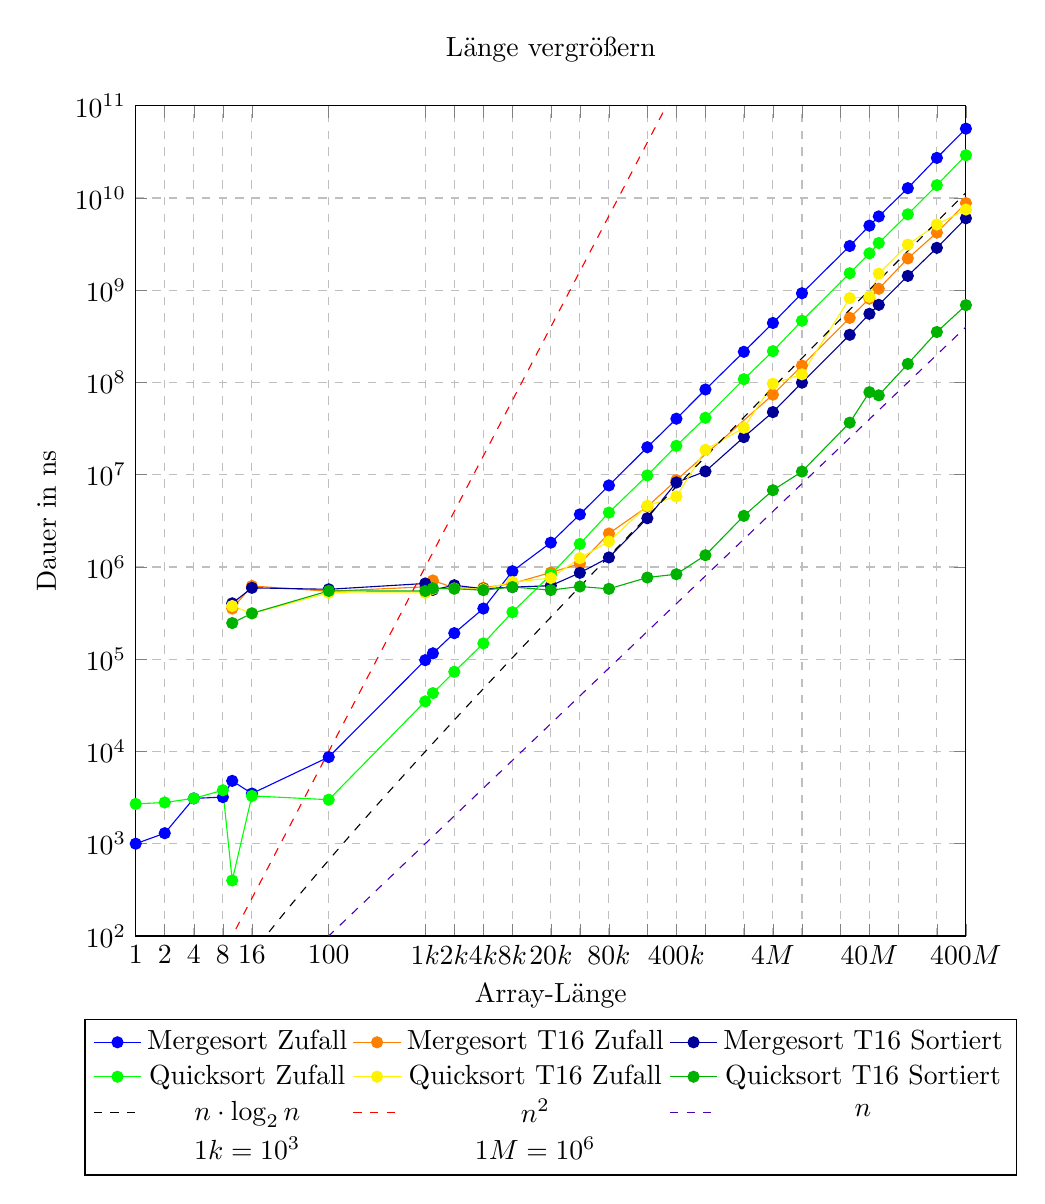
\begin{tikzpicture}
        \begin{axis}[
                title style={yshift=1.5ex},
                width=1\textwidth,
                height=1\textwidth,
                xlabel={Array-Länge},
                ylabel={Dauer in ns},
                title={Länge vergrößern},
                xmin=1, xmax=400000000,
                ymin=100, ymax=1*10^11,
                grid=both,
                grid style=dashed,
                % legend pos=south east,
                legend style={
                        at={(0.5,-0.1)},
                        anchor=north,
                        legend columns=3
                    },
                xmode=log,
                log basis x=10,
                %xtick=data,
                xtick={1,2,4,8,16,100,1000,2000,4000,8000,20000,40000,80000,200000,400000,800000,2000000,4000000,8000000,20000000,40000000,80000000,200000000,400000000},
                xticklabels={
                        $1$,$2$,$4$,$8$,$16$,
                        $100$,$1k$,
                        $2k$,$4k$,$8k$,
                        $20k$,$ $,$80k$,
                        $ $,$400k$,$ $,
                        $ $,$4M$,$ $,
                        $ $,$40M$,$ $,
                        $ $,$400M$,$ $
                    },
                ymode=log,
                log basis y=10,
                ytick={1,10,10^2,10^3,10^4,10^5,10^6,10^7,10^8,10^9,10^10,10^11},
                yticklabels={$1$,$10$,$10^{2}$,$10^{3}$,$10^{4}$,$10^{5}$,$10^{6}$,$10^{7}$,$10^{8}$,$10^{9}$,$10^{10}$,$10^{11}$}
                % scaled x ticks=false,
                % scaled y ticks=false,
            ]
            \MergesortgZufallG
            \MergesortZufallSechzehnThreads
            \MergesortSortiertSechzehnThreads
            % \MergesortFastSortiertSechzehnThreads
            \QuicksortZufallG
            \QuicksortZufallSechzehnThreads
            \QuicksortSortiertSechzehnThreads
            % \QuicksortFastSortiertSechzehnThreads
            % n*log2(n)
            \addplot[black, dashed,domain=1:400000000, samples=1000] {x*log2(x)};
            \addlegendentry{$n \cdot \log_2 n$}
            % n^2
            \addplot[red, dashed,domain=1:4e8, samples=100] {x*x};
            \addlegendentry{$n^2$}
            % n
            \addplot[blue!70!red, dashed,domain=1:4e8, samples=100] {x};
            \addlegendentry{$n$}
            \addlegendimage{empty legend}
            \addlegendentry{$1k = 10^3$}
            \addlegendimage{empty legend}
            \addlegendentry{$1M = 10^6$}
        \end{axis}
    \end{tikzpicture}%
}

\newcommand{\TiefenbasierteThreadErzeugungDiagrammB}{%
    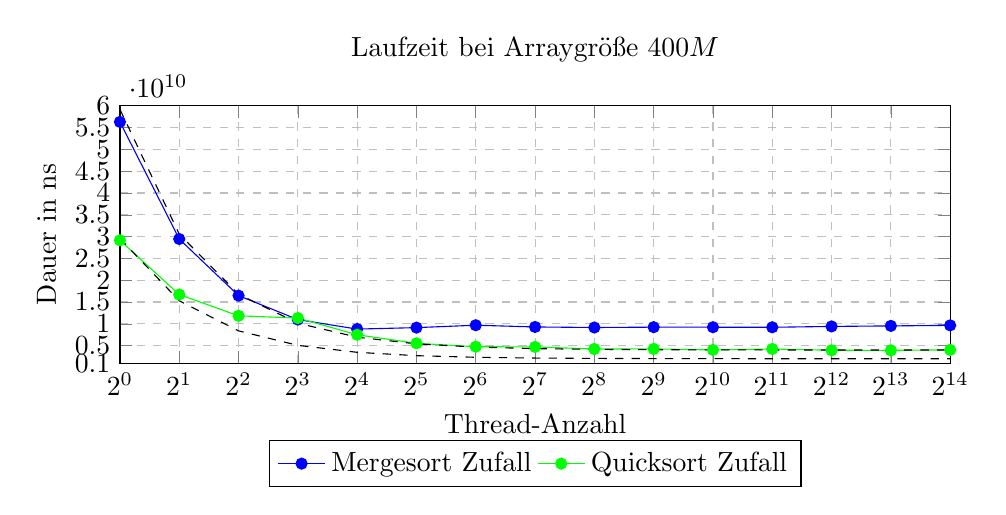
\begin{tikzpicture}
        \begin{axis}[
                title style={yshift=1.5ex},
                width=1\textwidth,
                height=0.4\textwidth,
                xlabel={Thread-Anzahl},
                ylabel={Dauer in ns},
                title={Laufzeit bei Arraygröße $400M$}, % Threads verdoppeln, Länge konstat, Strong Scaling
                xmin=1, xmax=2^14,
                ymin=1*10^9, ymax=6*10^10,
                grid=both,
                grid style=dashed,
                % legend pos=south east,
                legend style={
                        at={(0.5,-0.3)},
                        anchor=north,
                        legend columns=3
                    },
                xtick=data,
                % xtick={1},
                xmode=log,
                log basis x=2,
                % ymode=log,
                % log basis y=10,
                ytick={10^9,0.5*10^10,1*10^10,1.5*10^10,2*10^10,2.5*10^10,3*10^10,3.5*10^10,4*10^10,4.5*10^10,5*10^10,5.5*10^10,6*10^10},
                % scaled x ticks=false,
                % scaled y ticks=false,
            ]
            \MergesortZufallStrongScaling
            \QuicksortZufallStrongScaling
            \TheorieStrongScaling{400000000}{5}
            \TheorieStrongScaling{400000000}{2.5}
        \end{axis}
    \end{tikzpicture}%
}


\newcommand{\TiefenbasierteThreadErzeugungDiagrammC}{%
    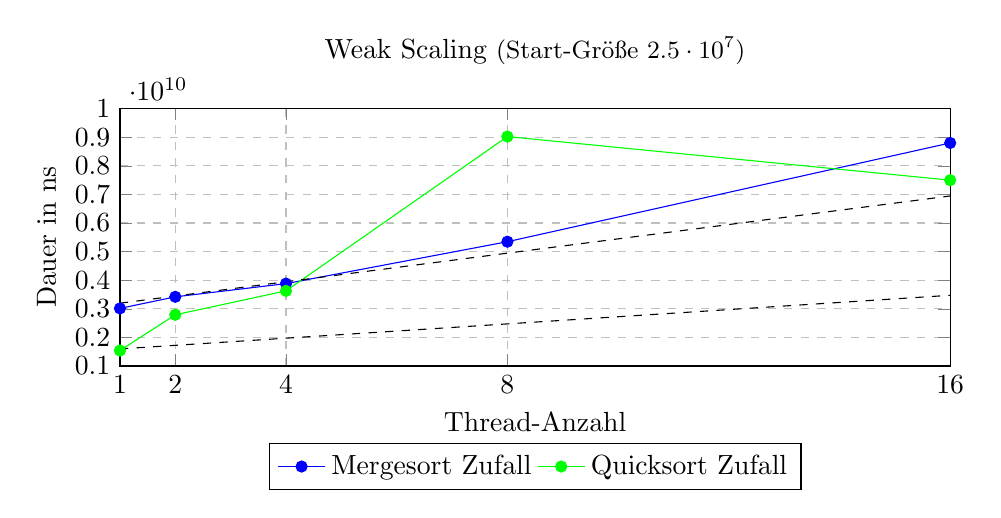
\begin{tikzpicture}
        \begin{axis}[
                title style={yshift=1.5ex},
                width=1\textwidth,
                height=0.4\textwidth,
                xlabel={Thread-Anzahl},
                ylabel={Dauer in ns},
                title={Weak Scaling {\small (Start-Größe $2.5 \cdot {10^7}$)}}, % Threads und Länge verdoppeln
                xmin=1, xmax=16,
                ymin=1*10^9, ymax=1*10^10,
                grid=both,
                grid style=dashed,
                % legend pos=south east,
                legend style={
                        at={(0.5,-0.3)},
                        anchor=north,
                        legend columns=3
                    },
                xtick=data,
                % xtick={1},
                % ymode=log,
                % log basis y=10,
                ytick={0.1*10^10,0.2*10^10,0.3*10^10,0.4*10^10,0.5*10^10,0.6*10^10,0.7*10^10,0.8*10^10,0.9*10^10,1*10^10},
                % scaled x ticks=false,
                % scaled y ticks=false,
            ]
            \MergesortZufallWeakScaling
            \QuicksortZufallWeakScaling
            \TheorieWeakScaling{5}
            \TheorieWeakScaling{2.5}
        \end{axis}
    \end{tikzpicture}%
}

\newcommand{\WorkerthreadsDiagrammA}{%
    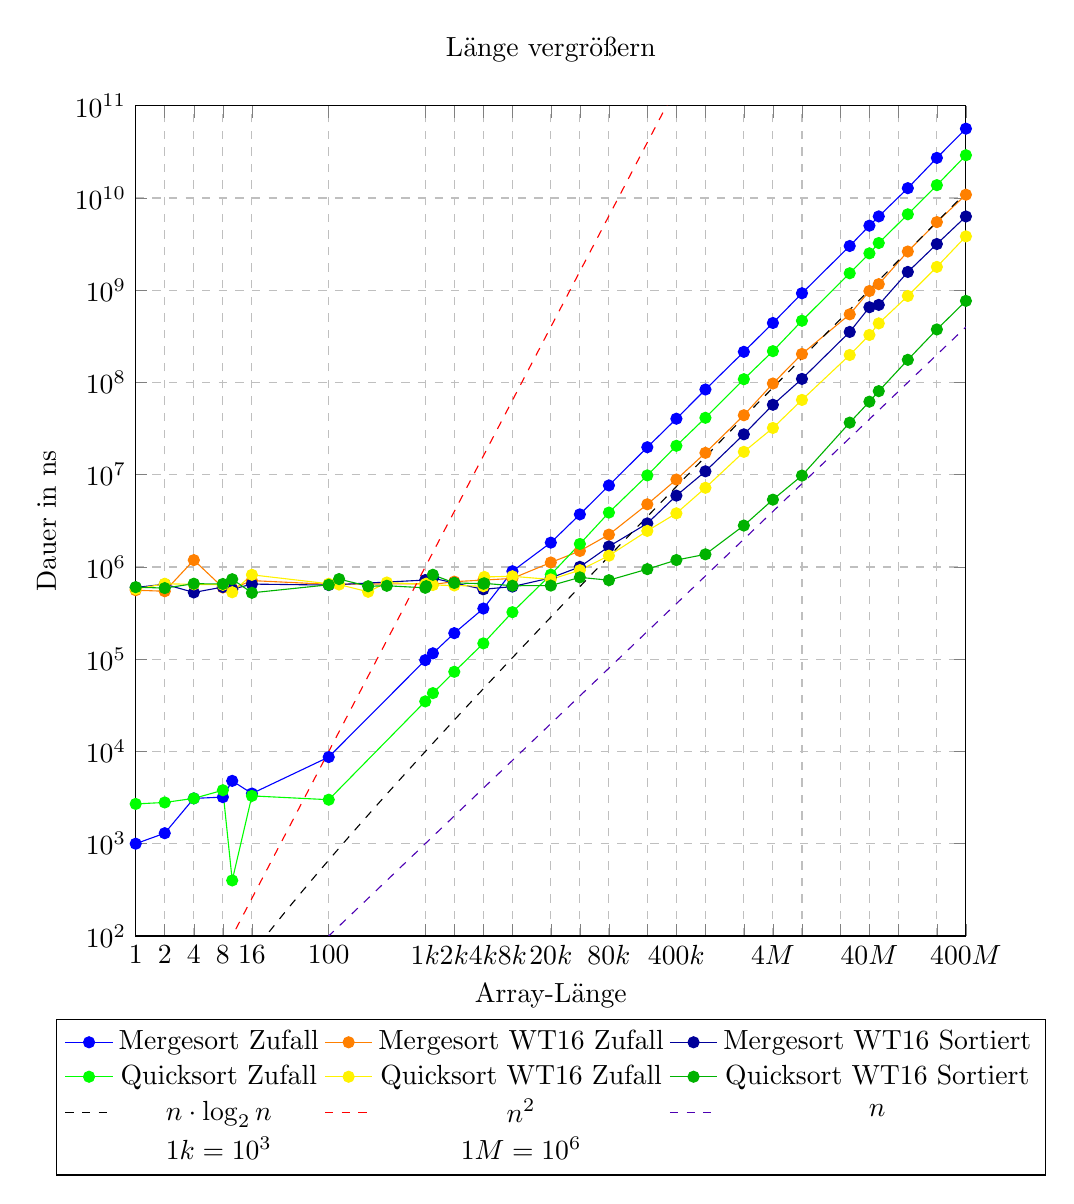
\begin{tikzpicture}
        \begin{axis}[
                title style={yshift=1.5ex},
                width=1\textwidth,
                height=1\textwidth,
                xlabel={Array-Länge},
                ylabel={Dauer in ns},
                title={Länge vergrößern},
                xmin=1, xmax=400000000,
                ymin=100, ymax=1*10^11,
                grid=both,
                grid style=dashed,
                % legend pos=south east,
                legend style={
                        at={(0.5,-0.1)},
                        anchor=north,
                        legend columns=3
                    },
                xmode=log,
                log basis x=10,
                %xtick=data,
                xtick={1,2,4,8,16,100,1000,2000,4000,8000,20000,40000,80000,200000,400000,800000,2000000,4000000,8000000,20000000,40000000,80000000,200000000,400000000},
                xticklabels={
                        $1$,$2$,$4$,$8$,$16$,
                        $100$,$1k$,
                        $2k$,$4k$,$8k$,
                        $20k$,$ $,$80k$,
                        $ $,$400k$,$ $,
                        $ $,$4M$,$ $,
                        $ $,$40M$,$ $,
                        $ $,$400M$,$ $
                    },
                ymode=log,
                log basis y=10,
                ytick={1,10,10^2,10^3,10^4,10^5,10^6,10^7,10^8,10^9,10^10,10^11},
                yticklabels={$1$,$10$,$10^{2}$,$10^{3}$,$10^{4}$,$10^{5}$,$10^{6}$,$10^{7}$,$10^{8}$,$10^{9}$,$10^{10}$,$10^{11}$}
                % scaled x ticks=false,
                % scaled y ticks=false,
            ]
            \MergesortgZufallG
            \MergesortZufallSechzehnWorkerThreads
            \MergesortSortiertSechzehnWorkerThreads
            \QuicksortZufallG
            \QuicksortZufallSechzehnWorkerThreads
            \QuicksortSortiertSechzehnWorkerThreads
            % n*log2(n)
            \addplot[black, dashed,domain=1:400000000, samples=1000] {x*log2(x)};
            \addlegendentry{$n \cdot \log_2 n$}
            % n^2
            \addplot[red, dashed,domain=1:4e8, samples=100] {x*x};
            \addlegendentry{$n^2$}
            % n
            \addplot[blue!70!red, dashed,domain=1:4e8, samples=100] {x};
            \addlegendentry{$n$}
            \addlegendimage{empty legend}
            \addlegendentry{$1k = 10^3$}
            \addlegendimage{empty legend}
            \addlegendentry{$1M = 10^6$}
        \end{axis}
    \end{tikzpicture}%
}

\newcommand{\WorkerthreadsDiagrammB}{%
    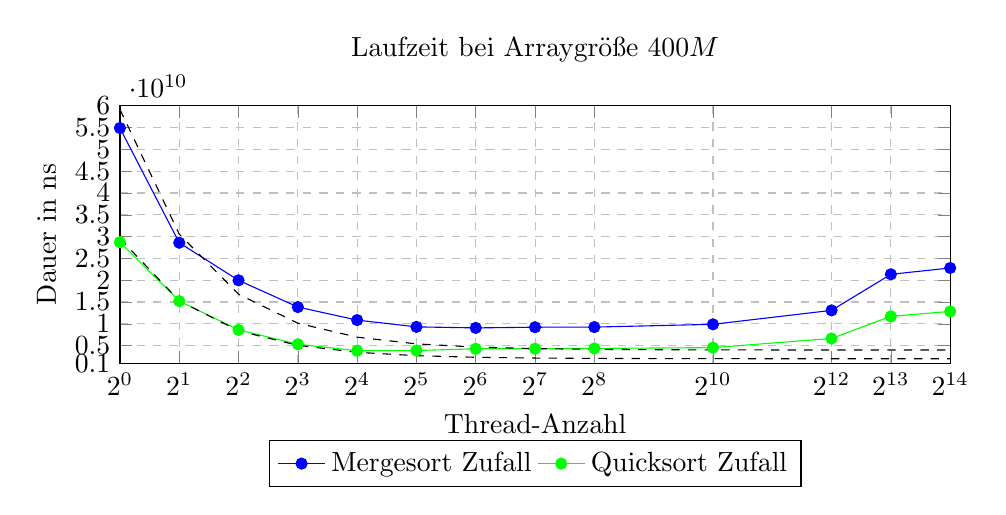
\begin{tikzpicture}
        \begin{axis}[
                title style={yshift=1.5ex},
                width=1\textwidth,
                height=0.4\textwidth,
                xlabel={Thread-Anzahl},
                ylabel={Dauer in ns},
                title={Laufzeit bei Arraygröße $400M$}, % Threads verdoppeln, Länge konstat, Strong Scaling
                xmin=1, xmax=16384,
                ymin=1*10^9, ymax=6*10^10,
                grid=both,
                grid style=dashed,
                % legend pos=south east,
                legend style={
                        at={(0.5,-0.3)},
                        anchor=north,
                        legend columns=3
                    },
                xtick=data,
                % xtick={1},
                xmode=log,
                log basis x=2,
                % ymode=log,
                % log basis y=10,
                ytick={10^9,0.5*10^10,1*10^10,1.5*10^10,2*10^10,2.5*10^10,3*10^10,3.5*10^10,4*10^10,4.5*10^10,5*10^10,5.5*10^10,6*10^10},
                % scaled x ticks=false,
                % scaled y ticks=false,
            ]
            \MergesortWZufallStrongScaling
            \QuicksortWZufallStrongScaling
            \TheorieStrongScaling{400000000}{5}
            \TheorieStrongScaling{400000000}{2.5}
        \end{axis}
    \end{tikzpicture}%
}


\newcommand{\WorkerthreadsDiagrammC}{%
    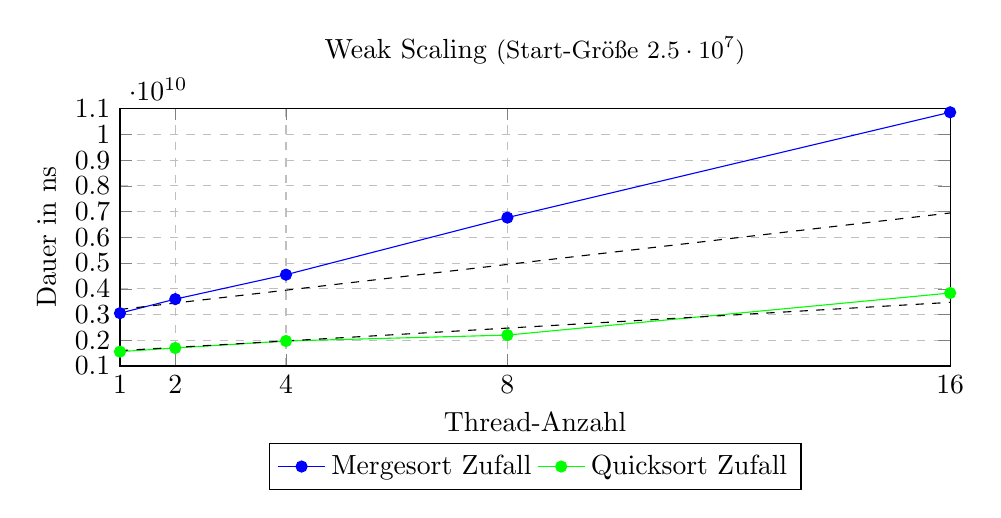
\begin{tikzpicture}
        \begin{axis}[
                title style={yshift=1.5ex},
                width=1\textwidth,
                height=0.4\textwidth,
                xlabel={Thread-Anzahl},
                ylabel={Dauer in ns},
                title={Weak Scaling {\small (Start-Größe $2.5 \cdot {10^7}$)}}, % Threads und Länge verdoppeln
                xmin=1, xmax=16,
                ymin=1*10^9, ymax=1.1*10^10,
                grid=both,
                grid style=dashed,
                % legend pos=south east,
                legend style={
                        at={(0.5,-0.3)},
                        anchor=north,
                        legend columns=3
                    },
                xtick=data,
                % xtick={1},
                % ymode=log,
                % log basis y=10,
                ytick={0.1*10^10,0.2*10^10,0.3*10^10,0.4*10^10,0.5*10^10,0.6*10^10,0.7*10^10,0.8*10^10,0.9*10^10,1*10^10,1.1*10^10},
                % scaled x ticks=false,
                % scaled y ticks=false,
            ]
            \MergesortWZufallWeakScaling
            \QuicksortWZufallWeakScaling
            \TheorieWeakScaling{5}
            \TheorieWeakScaling{2.5}
        \end{axis}
    \end{tikzpicture}%
}

\newcommand{\EinflussDesDatentypsDiagrammA}{%
    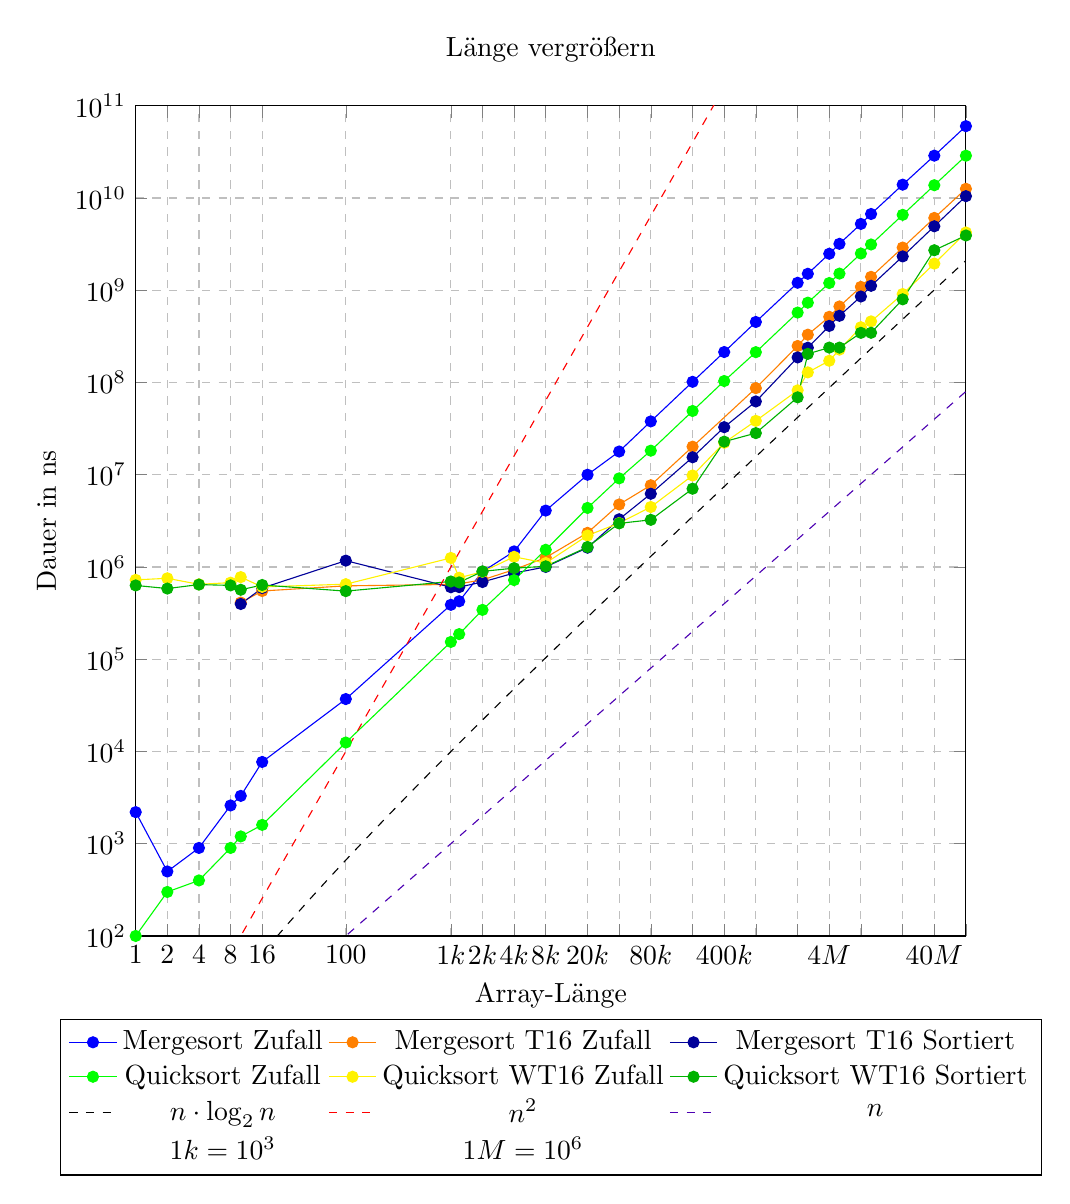
\begin{tikzpicture}
        \begin{axis}[
                title style={yshift=1.5ex},
                width=1\textwidth,
                height=1\textwidth,
                xlabel={Array-Länge},
                ylabel={Dauer in ns},
                title={Länge vergrößern},
                xmin=1, xmax=80000000,
                ymin=100, ymax=1*10^11,
                grid=both,
                grid style=dashed,
                % legend pos=south east,
                legend style={
                        at={(0.5,-0.1)},
                        anchor=north,
                        legend columns=3
                    },
                xmode=log,
                log basis x=10,
                %xtick=data,
                xtick={1,2,4,8,16,100,1000,2000,4000,8000,20000,40000,80000,200000,400000,800000,2000000,4000000,8000000,20000000,40000000,80000000,200000000,400000000},
                xticklabels={
                        $1$,$2$,$4$,$8$,$16$,
                        $100$,$1k$,
                        $2k$,$4k$,$8k$,
                        $20k$,$ $,$80k$,
                        $ $,$400k$,$ $,
                        $ $,$4M$,$ $,
                        $ $,$40M$,$ $,
                        $ $,$400M$,$ $
                    },
                ymode=log,
                log basis y=10,
                ytick={1,10,10^2,10^3,10^4,10^5,10^6,10^7,10^8,10^9,10^10,10^11},
                yticklabels={$1$,$10$,$10^{2}$,$10^{3}$,$10^{4}$,$10^{5}$,$10^{6}$,$10^{7}$,$10^{8}$,$10^{9}$,$10^{10}$,$10^{11}$}
                % scaled x ticks=false,
                % scaled y ticks=false,
            ]
            \MergesortStringZufallG
            \MergesortStringZufallSechzehnThreads
            \MergesortStringSortiertSechzehnThreads
            \QuicksortStringZufallG
            \QuicksortStringZufallSechzehnWorkerThreads
            \QuicksortStringSortiertSechzehnWorkerThreads
            % n*log2(n)
            \addplot[black, dashed,domain=1:400000000, samples=1000] {x*log2(x)};
            \addlegendentry{$n \cdot \log_2 n$}
            % n^2
            \addplot[red, dashed,domain=1:4e8, samples=100] {x*x};
            \addlegendentry{$n^2$}
            % n
            \addplot[blue!70!red, dashed,domain=1:4e8, samples=100] {x};
            \addlegendentry{$n$}
            \addlegendimage{empty legend}
            \addlegendentry{$1k = 10^3$}
            \addlegendimage{empty legend}
            \addlegendentry{$1M = 10^6$}
        \end{axis}
    \end{tikzpicture}%
}

\newcommand{\EinflussDesDatentypsDiagrammB}{%
    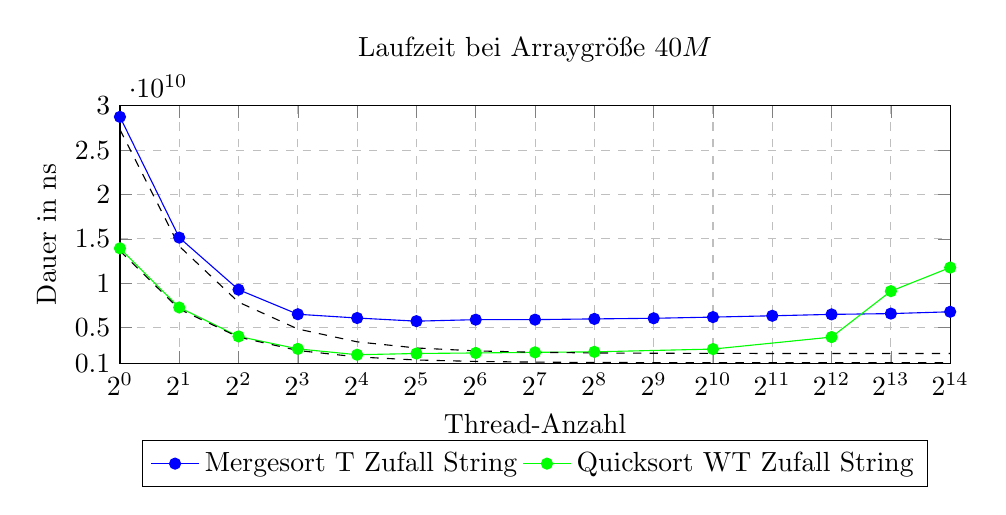
\begin{tikzpicture}
        \begin{axis}[
                title style={yshift=1.5ex},
                width=1\textwidth,
                height=0.4\textwidth,
                xlabel={Thread-Anzahl},
                ylabel={Dauer in ns},
                title={Laufzeit bei Arraygröße $40M$}, % Threads verdoppeln, Länge konstat, Strong Scaling
                xmin=1, xmax=16384,
                ymin=1*10^9, ymax=3*10^10,
                grid=both,
                grid style=dashed,
                % legend pos=south east,
                legend style={
                        at={(0.5,-0.3)},
                        anchor=north,
                        legend columns=3
                    },
                xtick=data,
                % xtick={1},
                xmode=log,
                log basis x=2,
                % ymode=log,
                % log basis y=10,
                ytick={10^9,0.5*10^10,1*10^10,1.5*10^10,2*10^10,2.5*10^10,3*10^10,3.5*10^10,4*10^10,4.5*10^10,5*10^10,5.5*10^10,6*10^10},
                % scaled x ticks=false,
                % scaled y ticks=false,
            ]
            \MergesortStringZufallStrongScaling
            \QuicksortWStringZufallStrongScaling
            \TheorieStrongScaling{40000000}{26}
            \TheorieStrongScaling{40000000}{13}
        \end{axis}
    \end{tikzpicture}%
}


\newcommand{\EinflussDesDatentypsDiagrammC}{%
    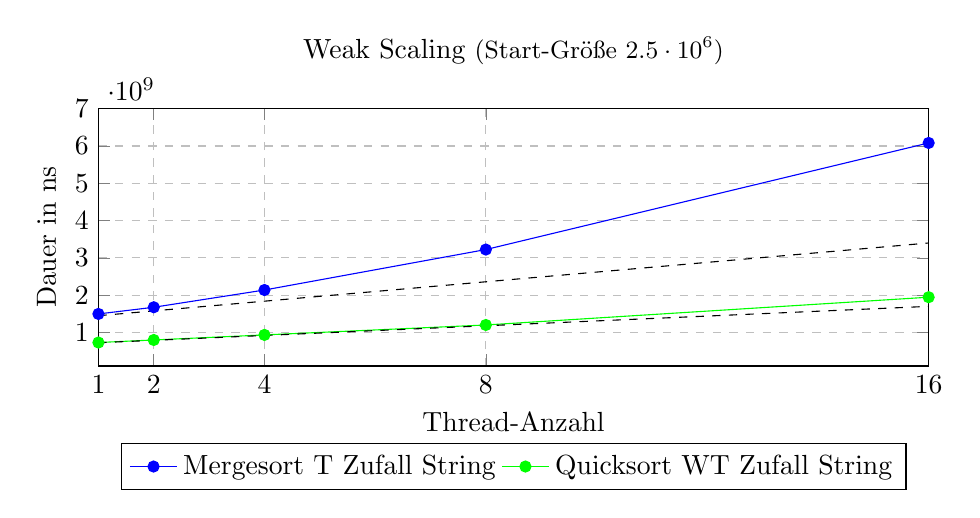
\begin{tikzpicture}
        \begin{axis}[
                title style={yshift=1.5ex},
                width=1\textwidth,
                height=0.4\textwidth,
                xlabel={Thread-Anzahl},
                ylabel={Dauer in ns},
                title={Weak Scaling {\small (Start-Größe $2.5 \cdot {10^6}$)}}, % Threads und Länge verdoppeln
                xmin=1, xmax=16,
                ymin=1*10^8, ymax=7*10^9,
                grid=both,
                grid style=dashed,
                % legend pos=south east,
                legend style={
                        at={(0.5,-0.3)},
                        anchor=north,
                        legend columns=3
                    },
                xtick=data,
                % xtick={1},
                % ymode=log,
                % log basis y=10,
                ytick={0.1*10^10,0.2*10^10,0.3*10^10,0.4*10^10,0.5*10^10,0.6*10^10,0.7*10^10,0.8*10^10,0.9*10^10,1*10^10},
                % scaled x ticks=false,
                % scaled y ticks=false,
            ]
            \MergesortStringZufallWeakScaling
            \QuicksortStringWZufallWeakScaling
            \TheorieWeakScalingB{26}
            \TheorieWeakScalingB{13}
        \end{axis}
    \end{tikzpicture}%
}

\newcommand{\initZeitenDiagrammA}{%
    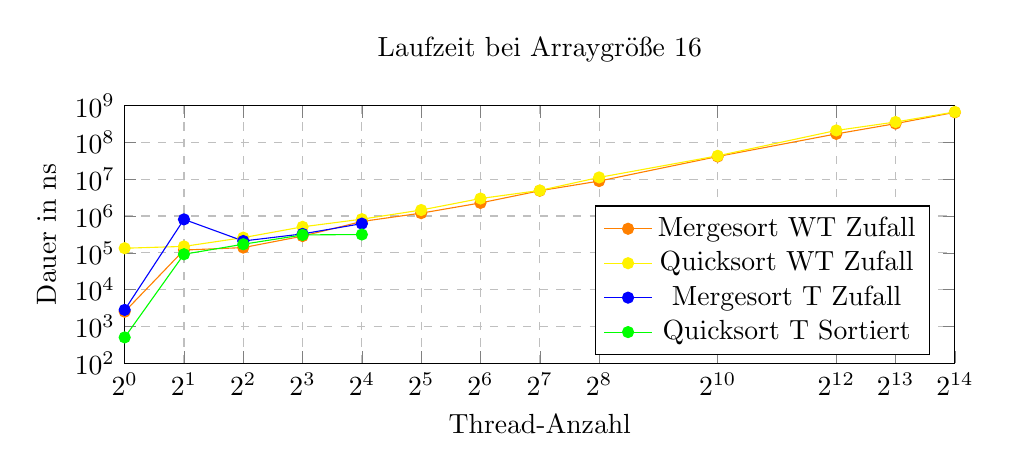
\begin{tikzpicture}
        \begin{axis}[
                title style={yshift=1.5ex},
                width=1\textwidth,
                height=0.4\textwidth,
                xlabel={Thread-Anzahl},
                ylabel={Dauer in ns},
                title={Laufzeit bei Arraygröße 16},
                grid=both,
                grid style=dashed,
                xmin=1, xmax=2^14,
                ymin=1*10^2, ymax=1*10^9,
                grid style=dashed,
                legend pos=south east,
                xtick=data,
                xmode=log,
                log basis x=2,
                ymode=log,
                log basis y=10,
                ytick={1*10^2,1*10^3,1*10^4,1*10^5,1*10^6,1*10^7,1*10^8,1*10^9},
            ]
            \MergesortWTInitZeiten
            \QuicksortWTInitZeiten
            \MergesortTInitZeiten
            \QuicksortTInitZeiten
        \end{axis}
    \end{tikzpicture}%
}